\section{Auswertung}
\label{sec:Auswertung}

Zunächst wurden die Zylinder ausgemessen. Insgesamt gab es vier verschiedene Zylinder, die gegebenenfalls auch gestapelt wurden.
Die folgenden Größen wurden für die Acrylobjekte mit einer Schieblehre ermittelt:
\begin{align*}
  z_1 &= 0.0404 \unit\meter & z_2 &= 0.0615 \unit\meter \\
  z_3 &= 0.0805 \unit\meter & z_2 &= 0.1205 \unit\meter \\
  d_\text{Platte} &= 0.006 \unit\meter
\end{align*}

\subsection{Schallgeschwindigkeit mittels des Impuls-Echo-Verfahren}

\subsection{Untersuchung des Augenmodells}

Die entsprechende Messung zu der Vermessung des Augenmodells ist in \autoref{fig:auge} dargestellt
und es sind fünf Peaks zu erkennen. Dabei ist der erste Peak zu vernachlässigen.
Aus der Messung lassen sich dann die Messdaten in \autoref{tab:auge} ablesen.
Dabei werden die Peaks den folgenden Bestandteilen des Auges zugeordnet:
\begin{align*}
  \text{Peak 1} &\to \text{Hornhaut} \\
  \text{Peak 2} &\to \text{Anfang der Linse} \\
  \text{Peak 3} &\to \text{Ende der Linse} \\
  \text{Peak 4} &\to \text{Netzhaut}
\end{align*}
Mit den Schallgeschwindigkeiten $c_L = 2500 \unit{\meter / \second}$ und $c_GK = 1410 \unit{\meter / \second}$.
Aus der allgemeinen Formel \ref{tbd} ergeben sich dann
\begin{align*}
  s_1 &= \frac{1}{2} c_GK t_1 = tbd \\
  s_2 &= \frac{1}{2} c_L t_2 = tbd \\
  s_3 &= \frac{1}{2} c_GK t_3 = tbd
\end{align*}


\begin{table}
  \centering
  \caption{Messdaten der Vermessung des Auges.}
  \label{tab:auge}
  \begin{tabular}{c c}
      \toprule
      Peak Nummer & $\frac{\unit\second} {\unit{\micro\second}}$ \\ 
      \midrule
      1 & 12 \\
      2 & 16 \\
      3 & 23 \\
      4 & 77 \\
      \bottomrule
  \end{tabular}
\end{table}

\begin{figure}
  \centering
  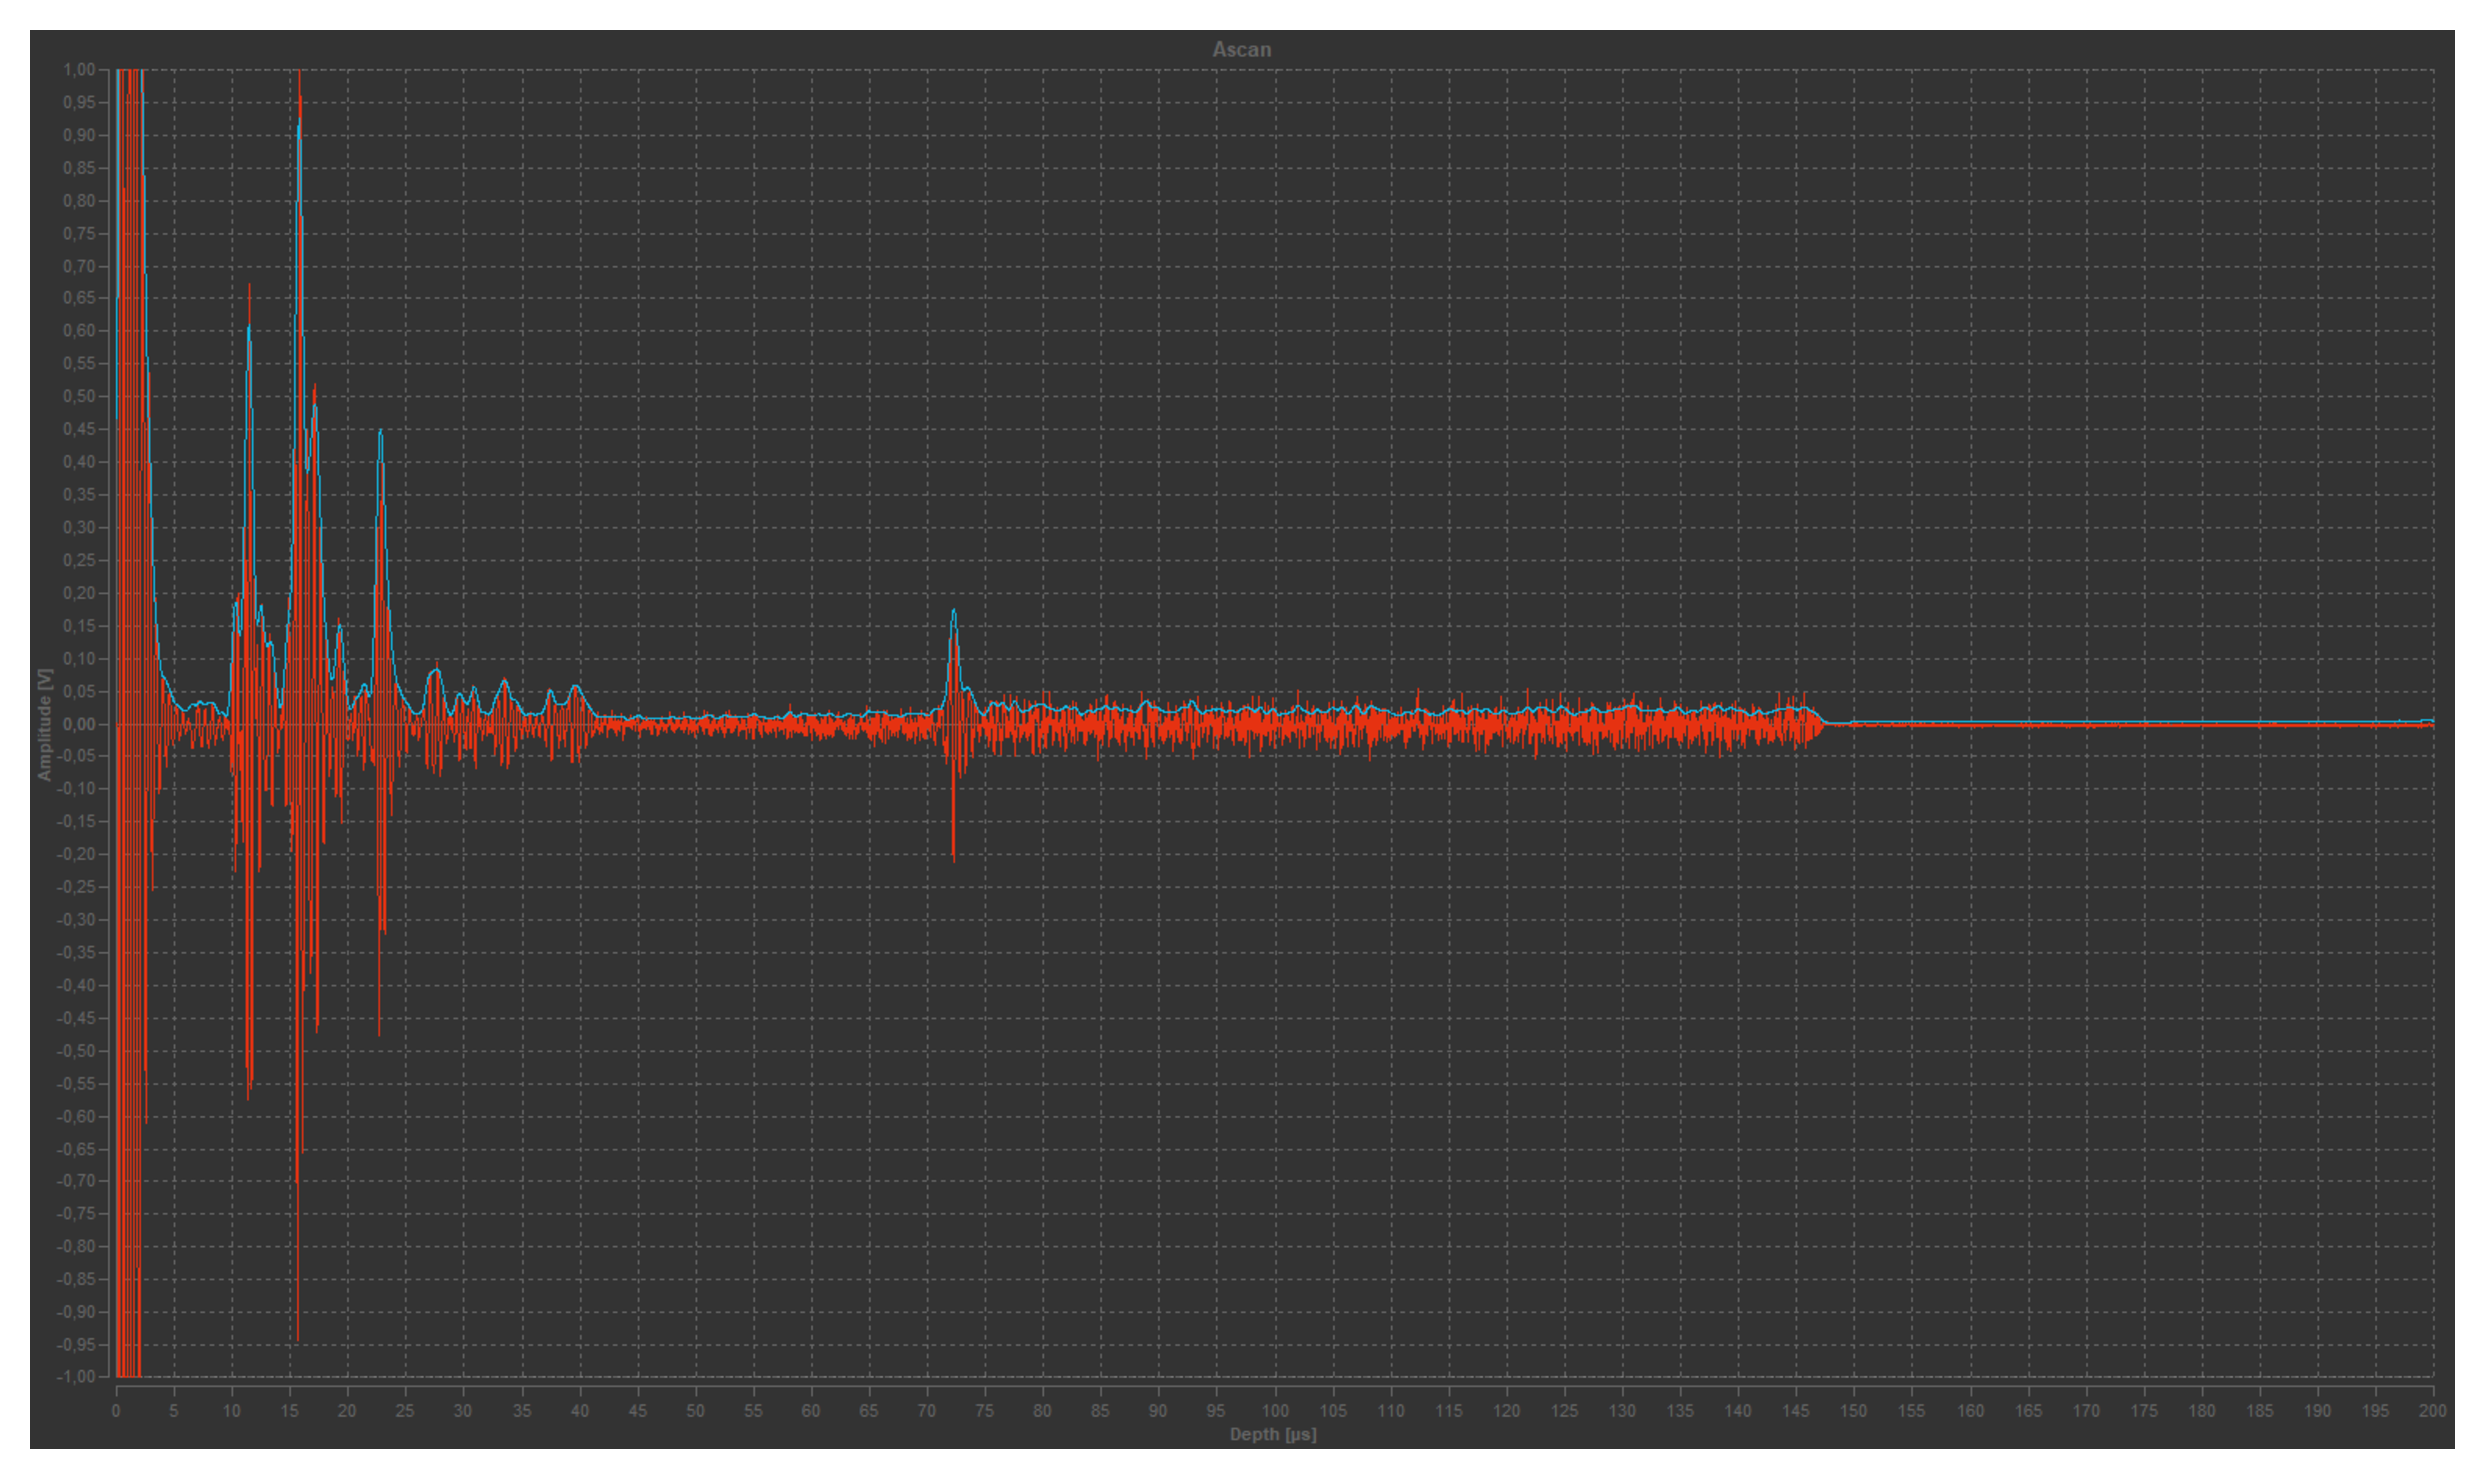
\includegraphics[width = 0.8\linewidth]{pictures/auge/Messung1Auge.pdf}
  \caption{Screenshot der Messung des Augenmodells}
  \label{fig:auge}
\end{figure}